\chapter{Packet structure}
\thispagestyle{empty}% no page number in chapter title page
\begin{table}[htbp]
\break
\setlength{\arrayrulewidth}{1mm}
\setlength{\tabcolsep}{12pt}
\renewcommand{\arraystretch}{1.5}
 {\rowcolors{3}{whitesmoke}{silver}
\begin{tabular}{ |p{3cm}|p{2cm}|p{8cm}|  }
\hline
\multicolumn{3}{|c|}{Packet Structure} \\
\hline
Content & Bytes & Description \\
\hline
Ethernet Header & 0 - 13 & Header due to packaging. \\
IPv4 Header & 14 - 33 & Header due to packaging. \\
UDP Header & 34 - 41 & Header due to packaging. \\
Frame Identifier & 42 - 45 & Binary variable coded as integer, either \textit{keyframe} or not. \\
Frame Number & 46 - 49 & Used to monitor that order of packages is not scrambled. Coded as integer. \\
Segment Number & 50 - 53 & Can be kept track of to detect any drops, coded as an integer. \\
Packet Size & 54 - 57 & For most packets it equals 1538 bites. Coded as long. \\
Event Occurred & 58 - 61 & Uninteresting for our purposes. Coded as float. \\
Sampling time & 62 - 65 & Same as above. Coded as a float. \\
Dummy Data & 66 onward & Necessary filler to achieve specified length. Filled with zeroes. \\
\hline
\end{tabular}
}
\caption{Breakdown of packet structure by byte}
\end{table}

\chapter{Other test results}
\thispagestyle{empty}

\clearpage

\section{No Cross-traffic}

\begin{figure}[!h]
\centering
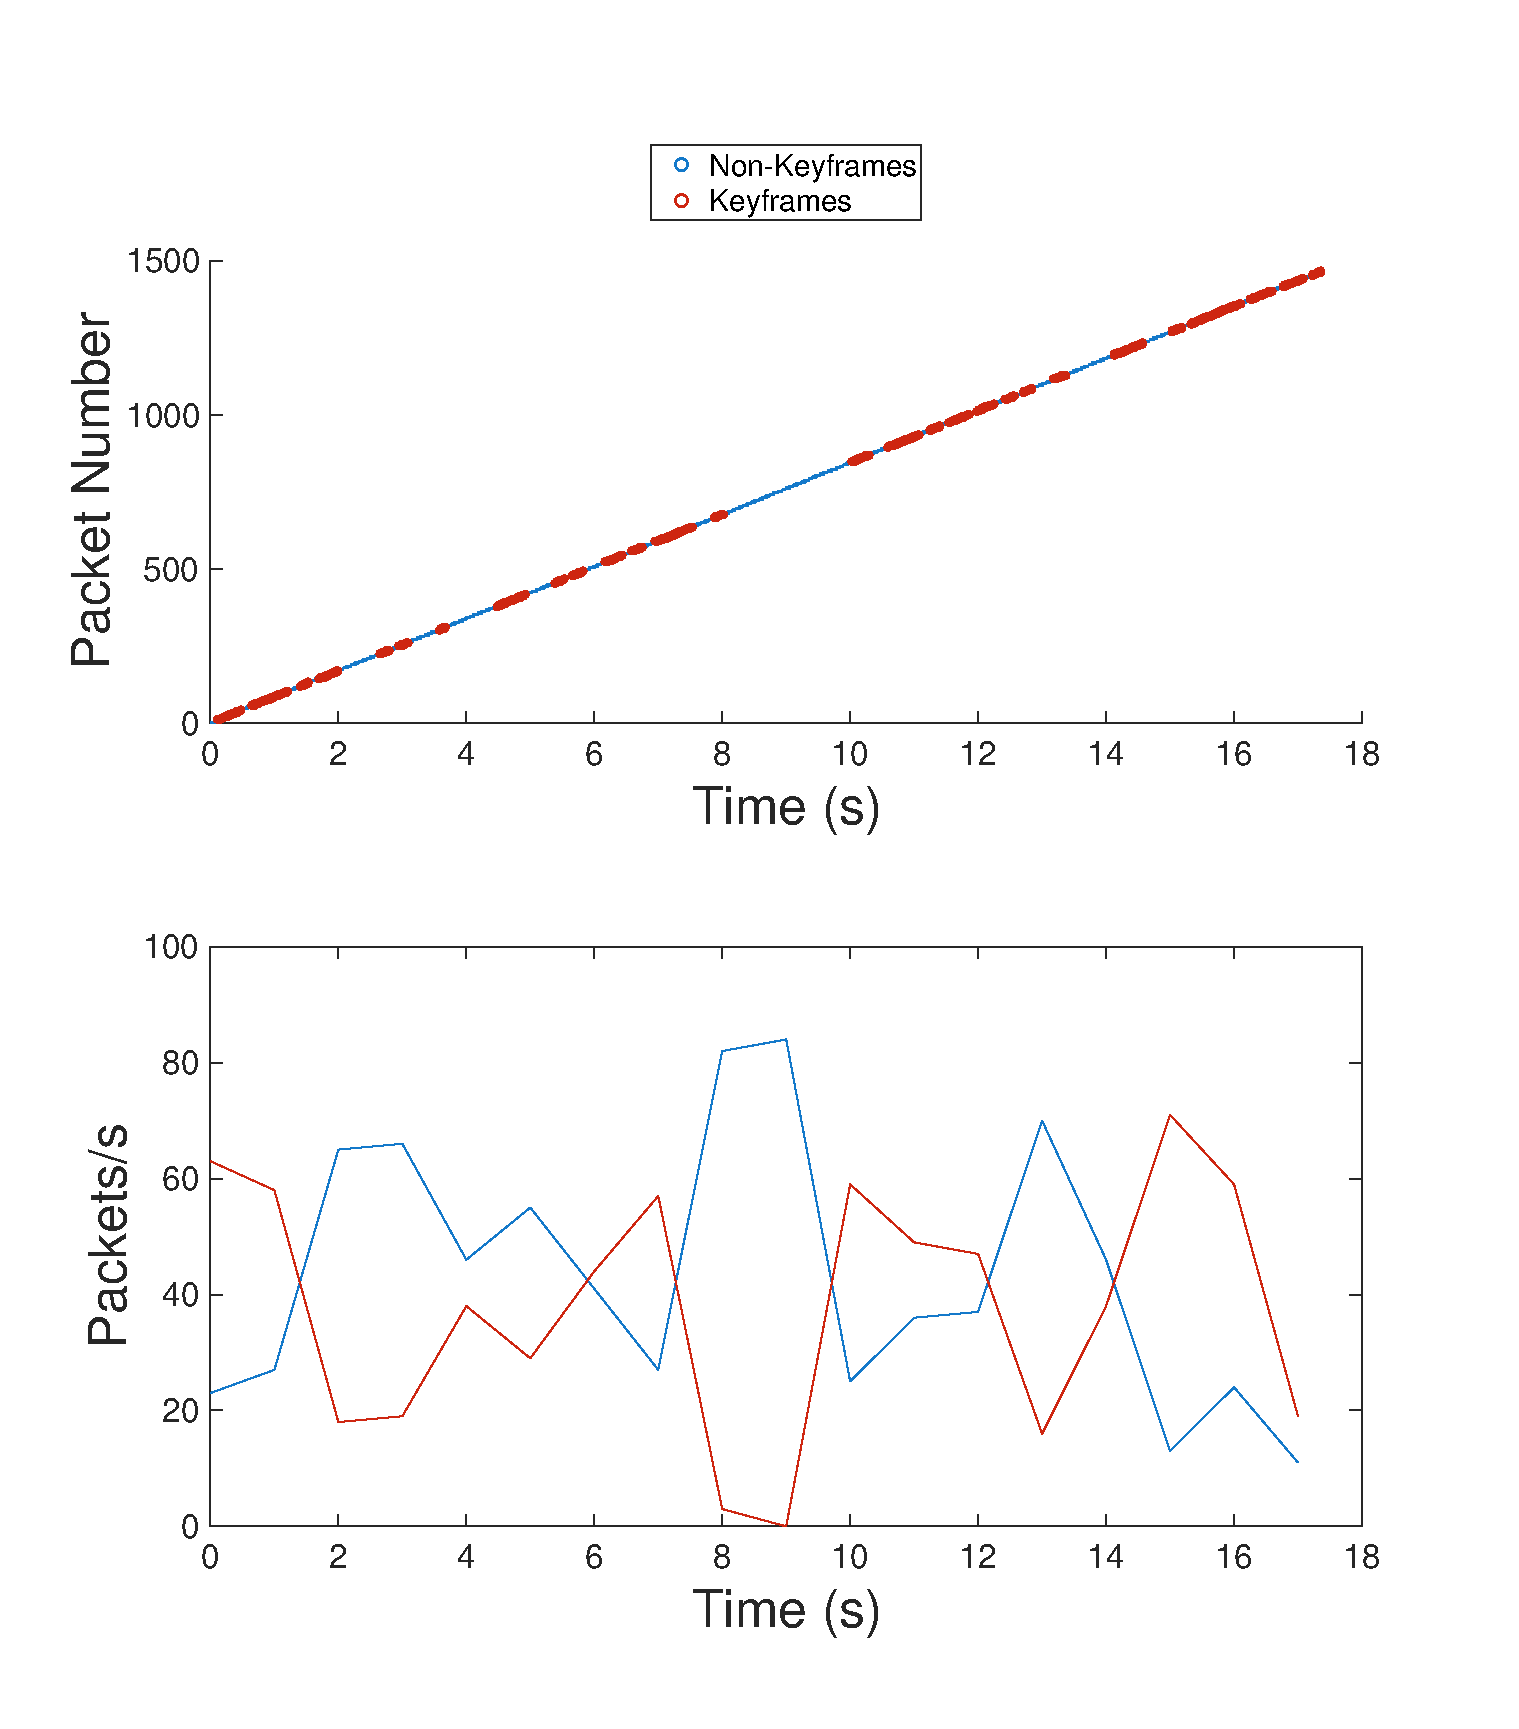
\includegraphics[scale = 0.55]{nocross_slow_1_4}
\caption{No cross-traffic ; Slow Channel (Path A : 1 Mbps, Path B : 4 Mbps), measured at the end of Path B}
\end{figure}
\clearpage

\begin{figure}[!h]
\centering
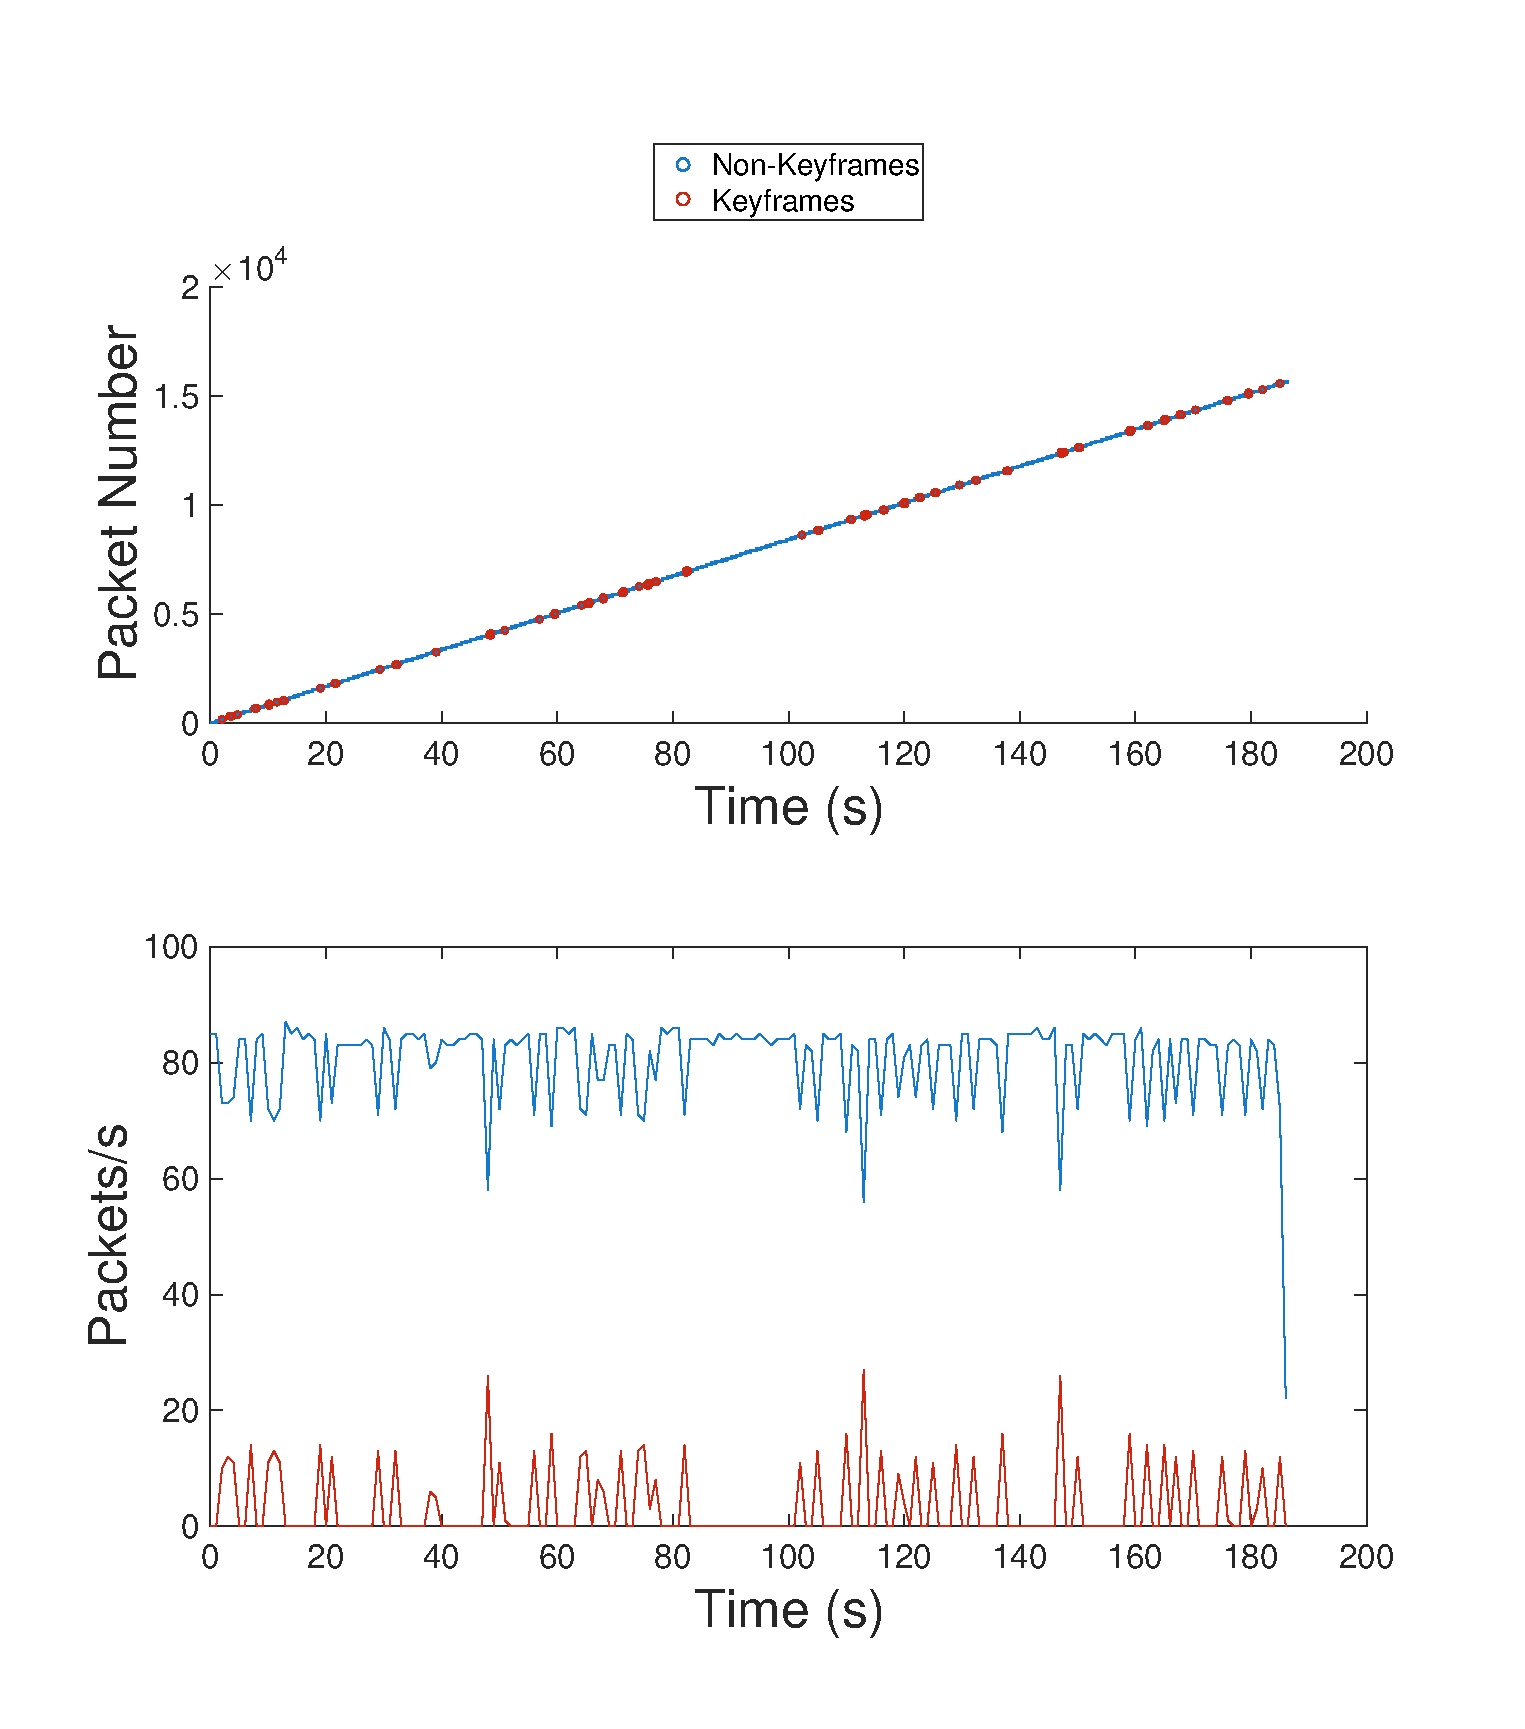
\includegraphics[scale = 0.55]{nocross_med_1_4}
\caption{No cross-traffic ; Medium Channel (Path A : 1 Mbps, Path B : 4 Mbps), measured at the end of Path B}
\end{figure}



\begin{figure}[!h]
\centering
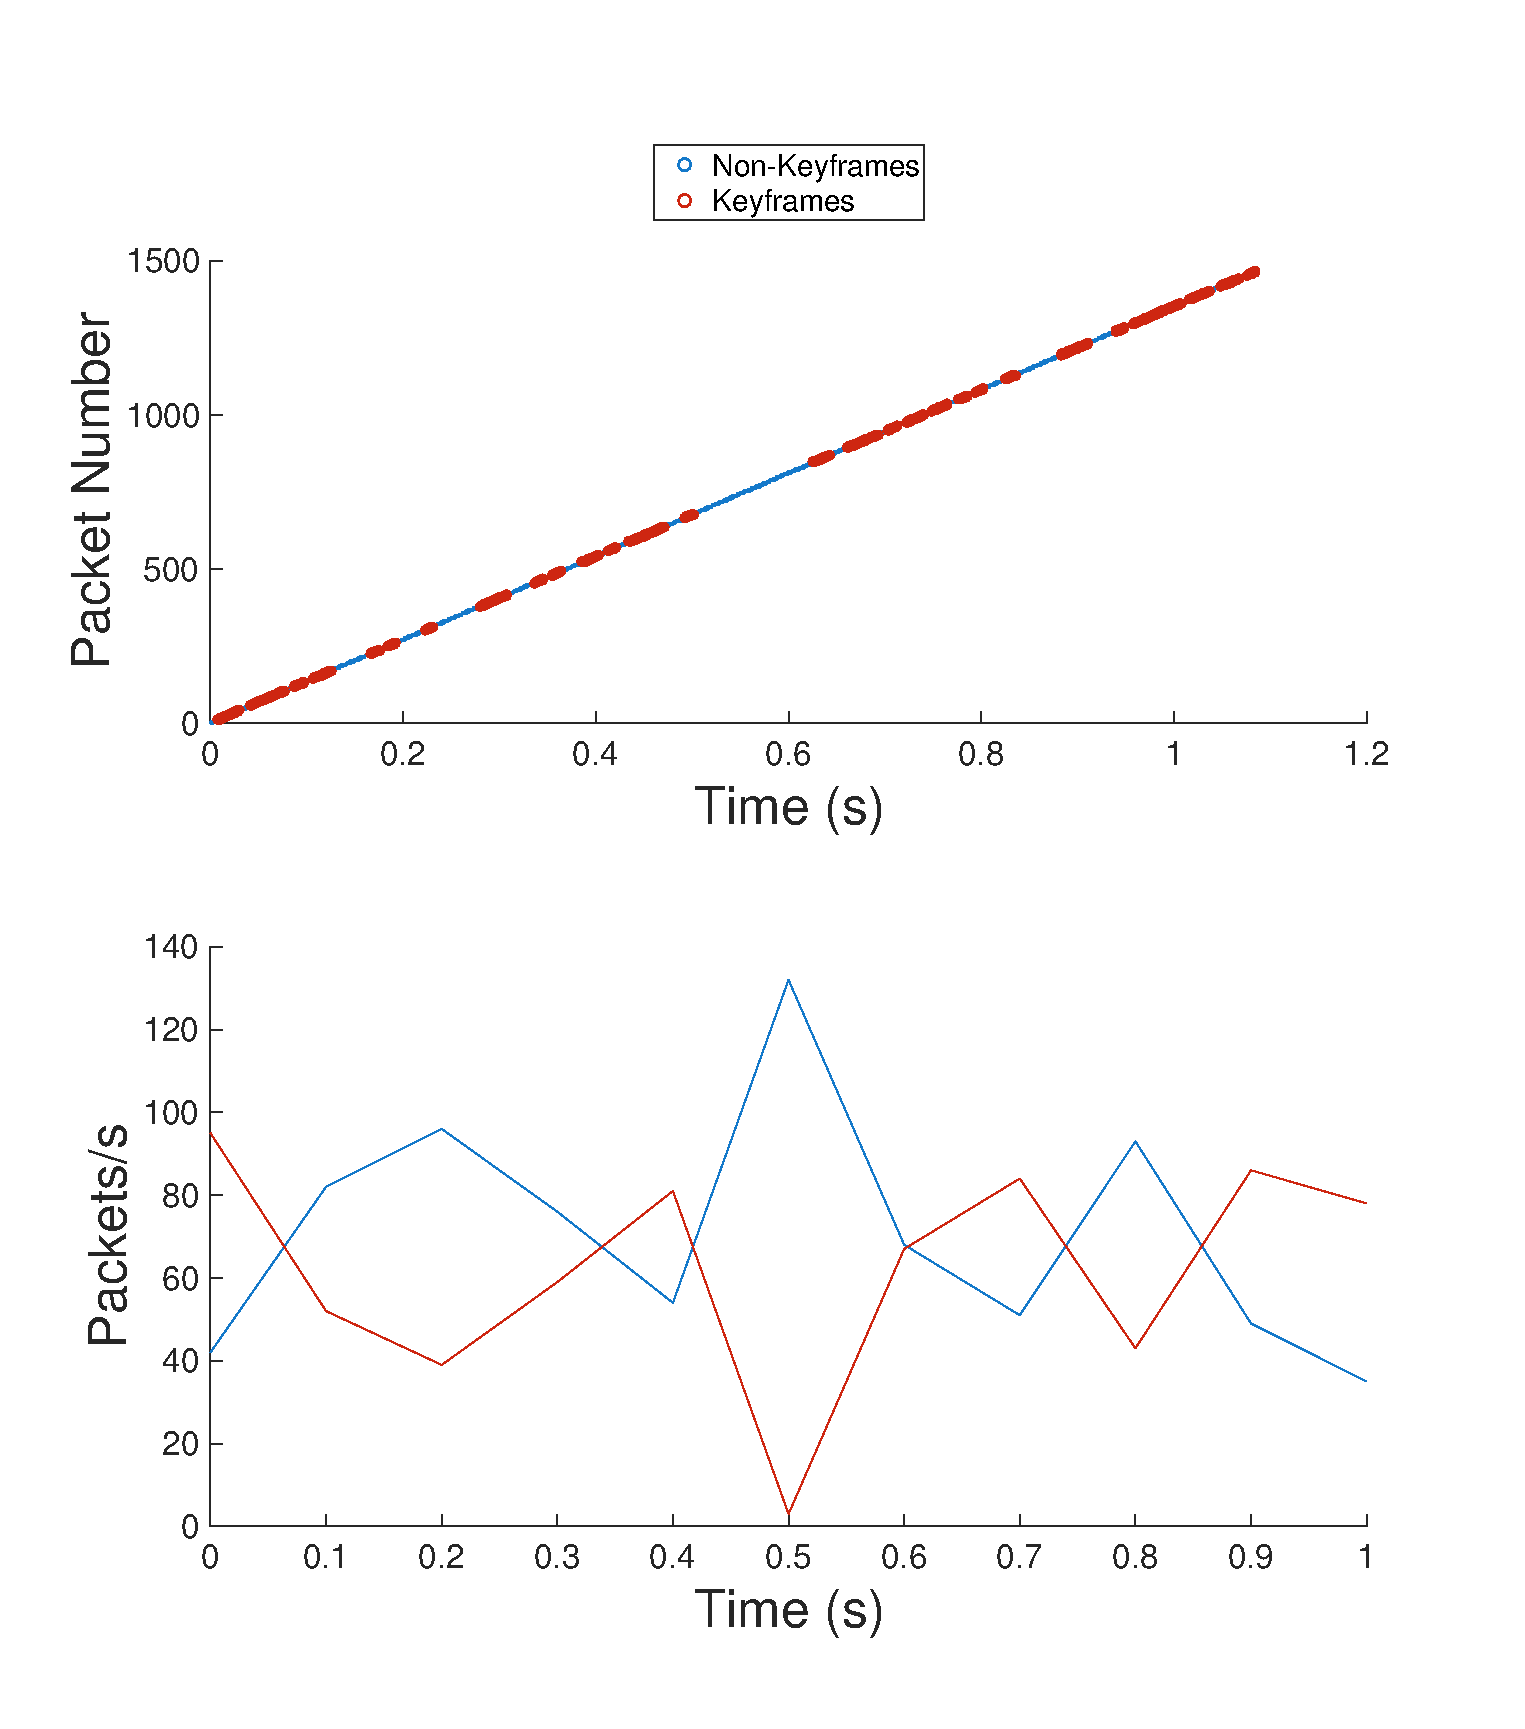
\includegraphics[scale = 0.55]{nocross_slow_16_16}
\caption{No cross-traffic ; Slow Channel (Path A : 16 Mbps, Path B : 16 Mbps), measured at the end of Path B}
\end{figure}

\begin{figure}[!h]
\centering
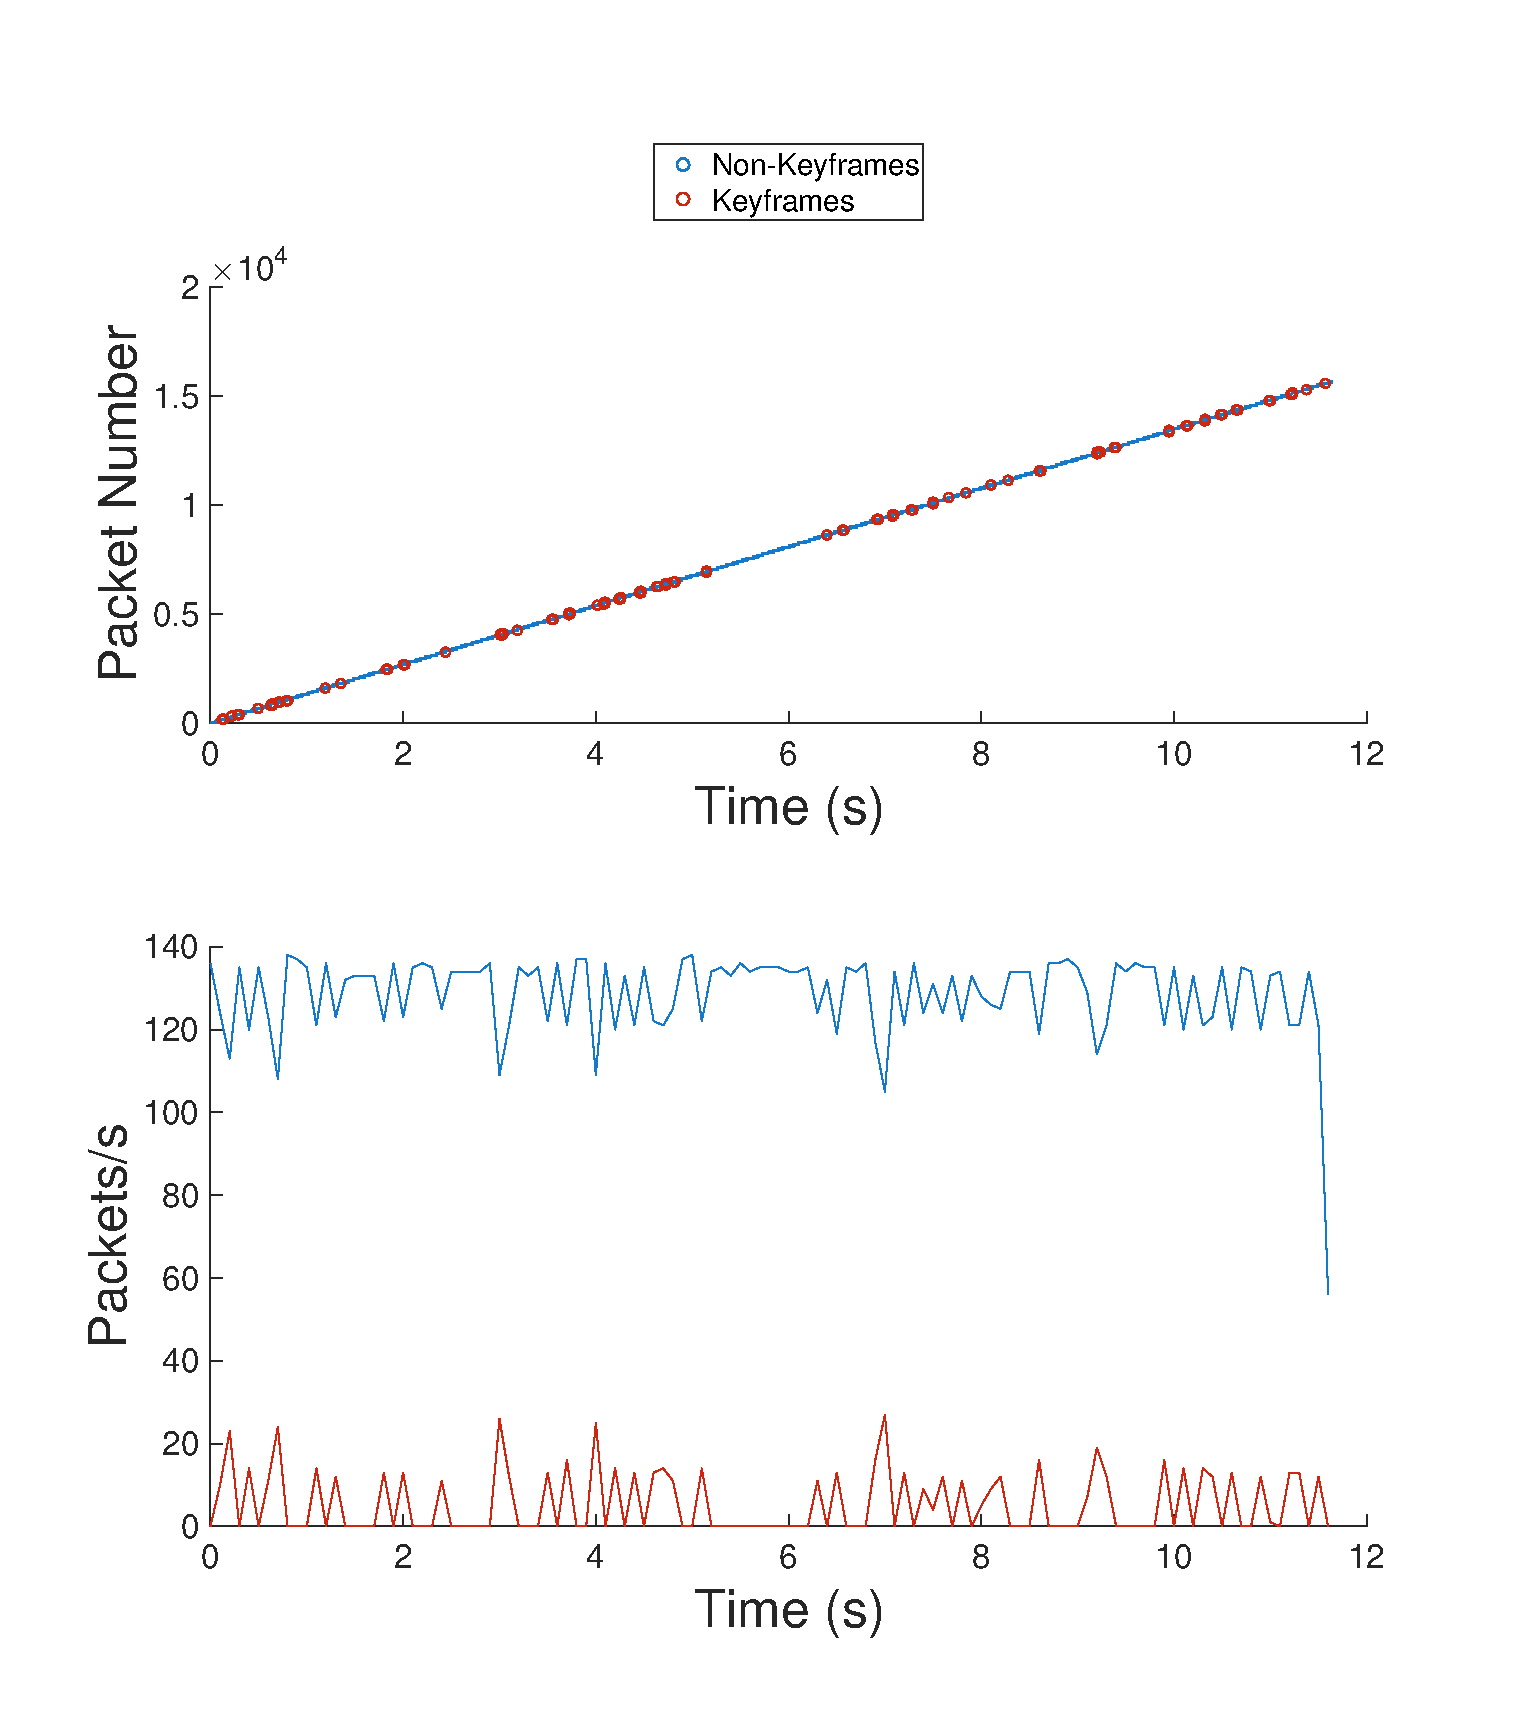
\includegraphics[scale = 0.55]{nocross_med_16_16}
\caption{No cross-traffic ; Medium Channel (Path A : 16 Mbps, Path B : 16 Mbps), measured at the end of Path B}
\end{figure}

\clearpage

\section{Random Cross-traffic}

\begin{figure}[!h]
\centering
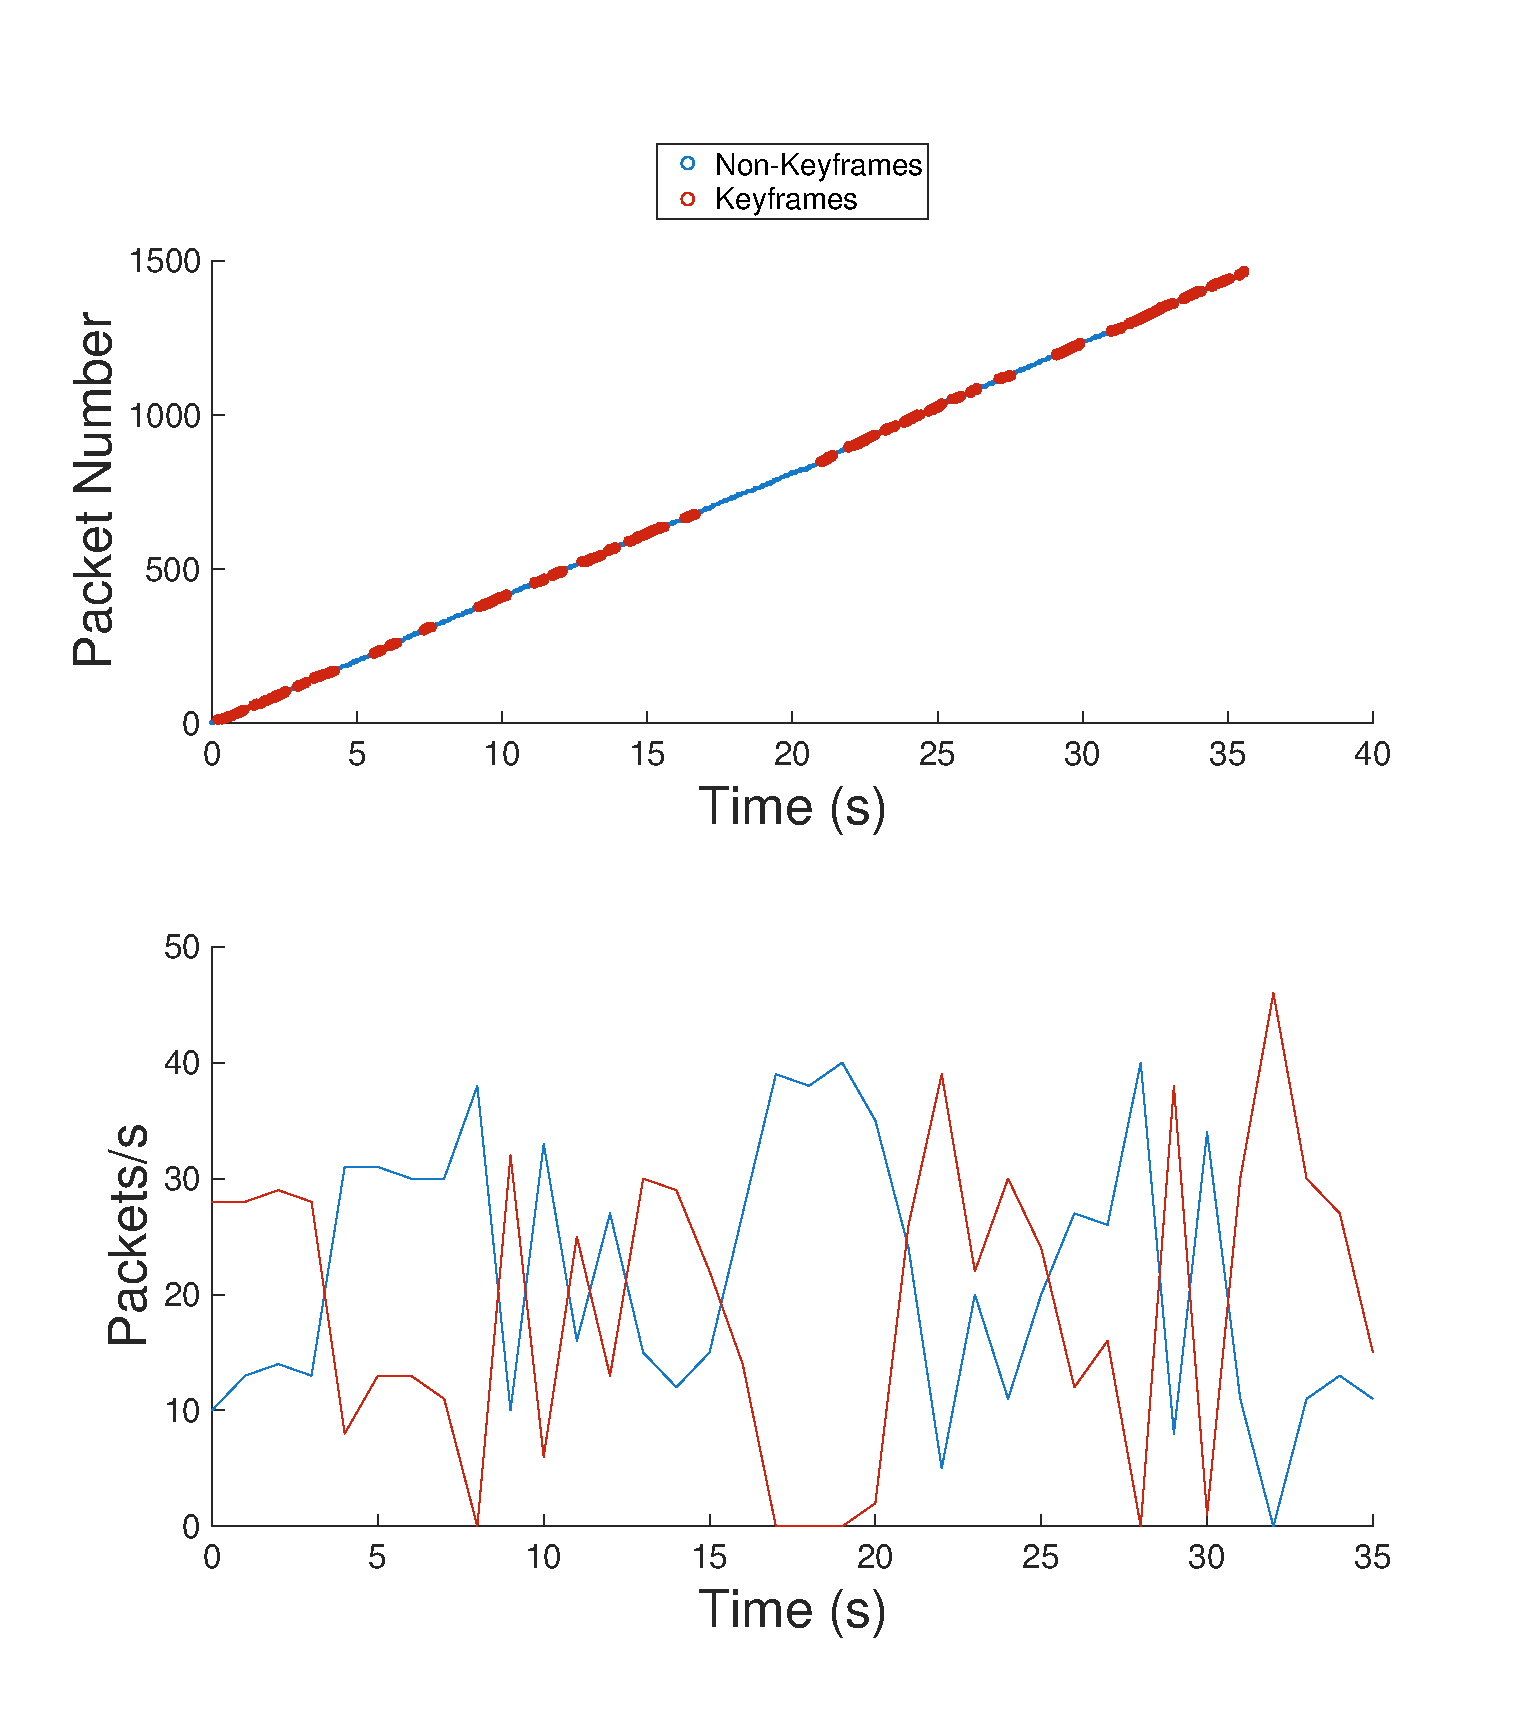
\includegraphics[scale = 0.55]{rand_slow_1_4_50}
\caption{Random cross-traffic ; Slow Channel (Path A : 4 Mbps, Path B : 1 Mbps), 50\% channel occupation, measured at the end of Path B}
\end{figure}
\clearpage

\begin{figure}[!h]
\centering
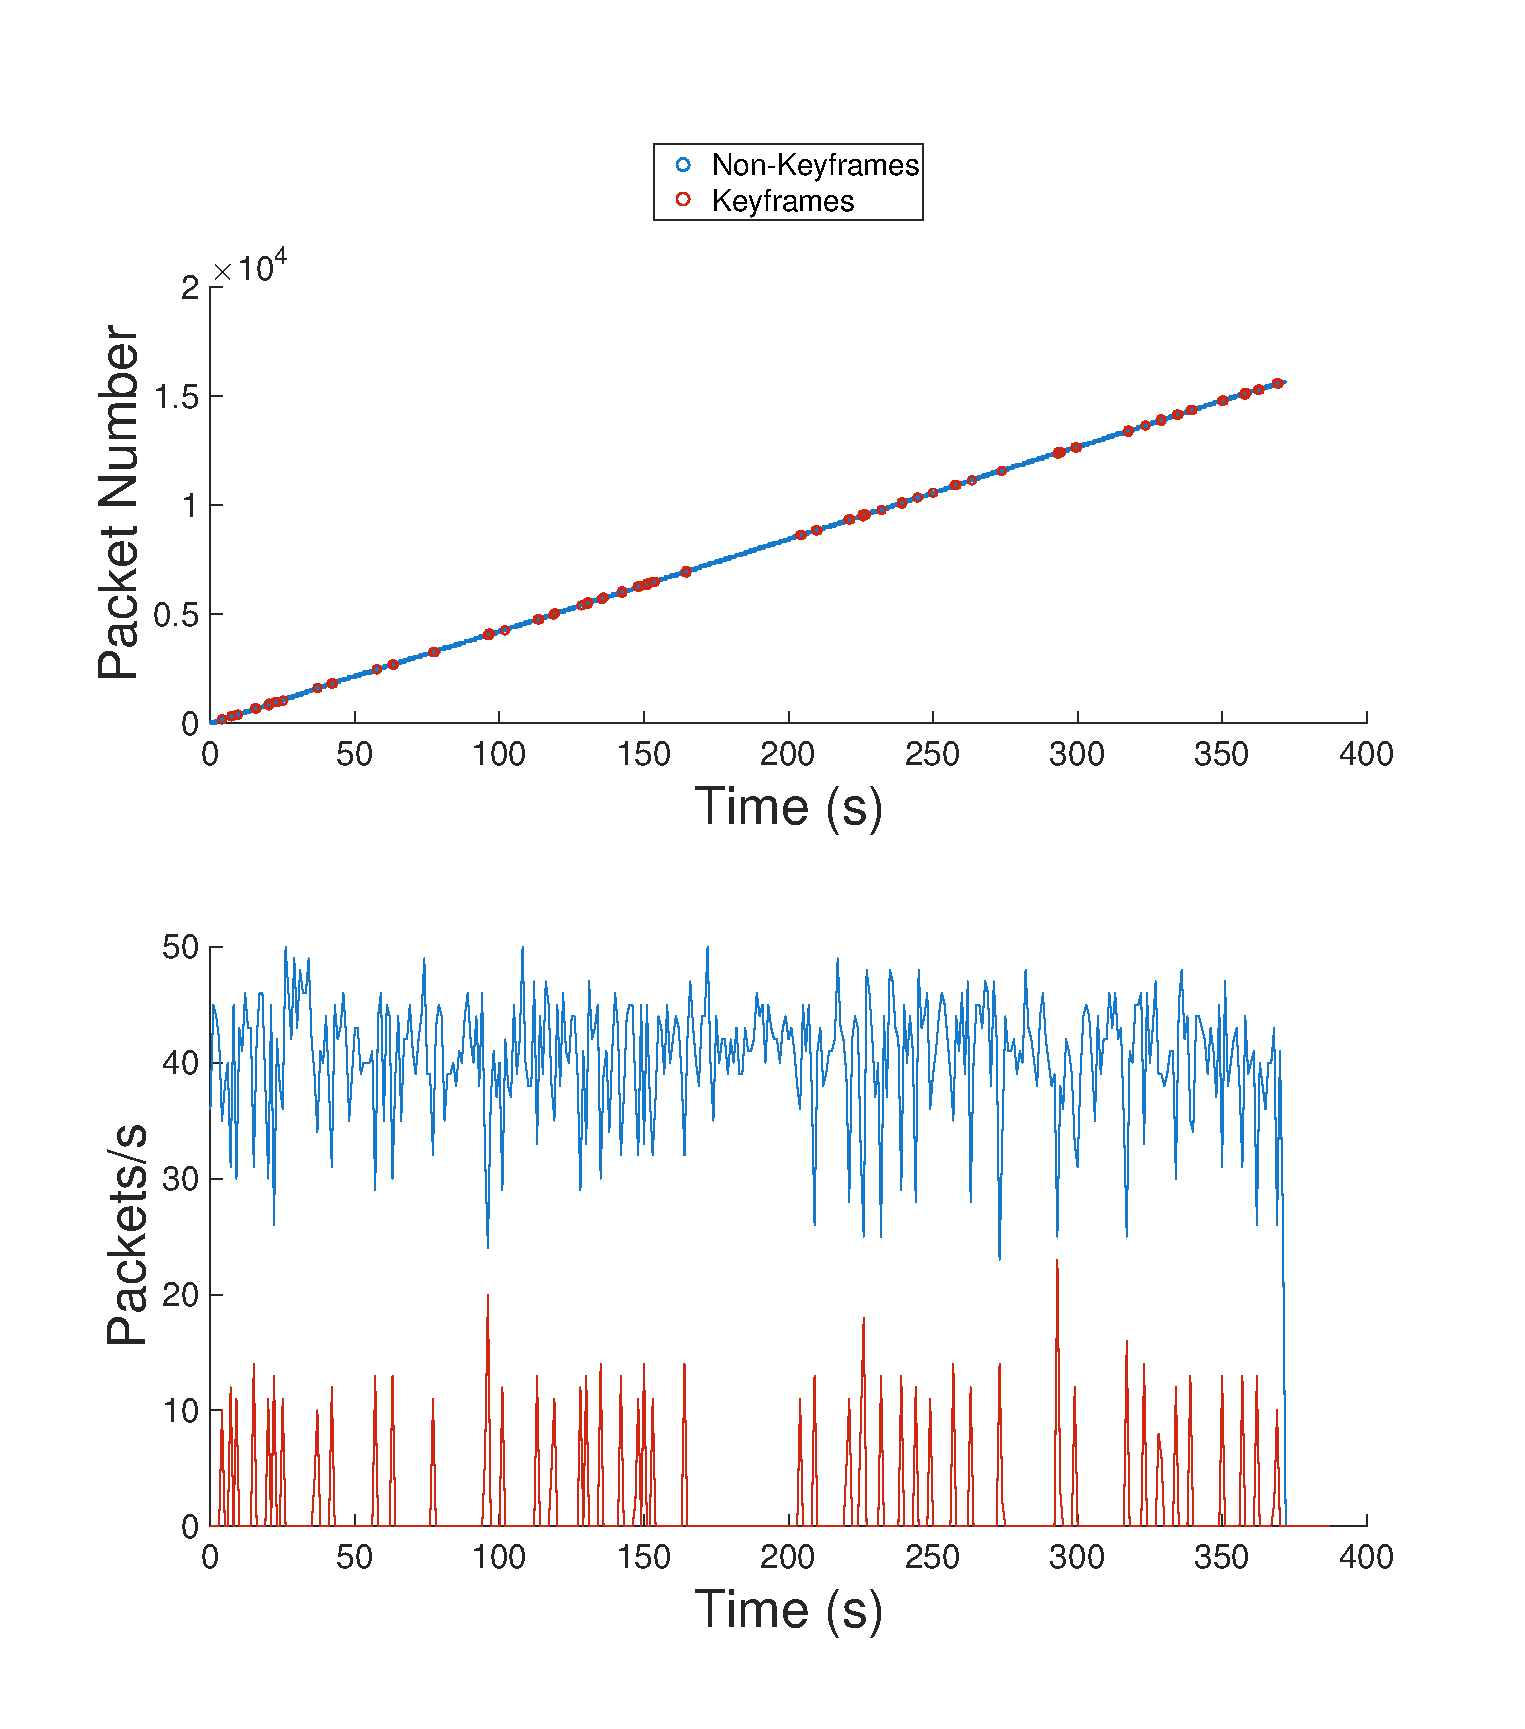
\includegraphics[scale = 0.55]{rand_med_1_4_50}
\caption{Random cross-traffic ; Medium Channel (Path A : 4 Mbps, Path B : 1 Mbps), 50\% channel occupation, measured at the end of Path B}
\end{figure}

\begin{figure}[!h]
\centering
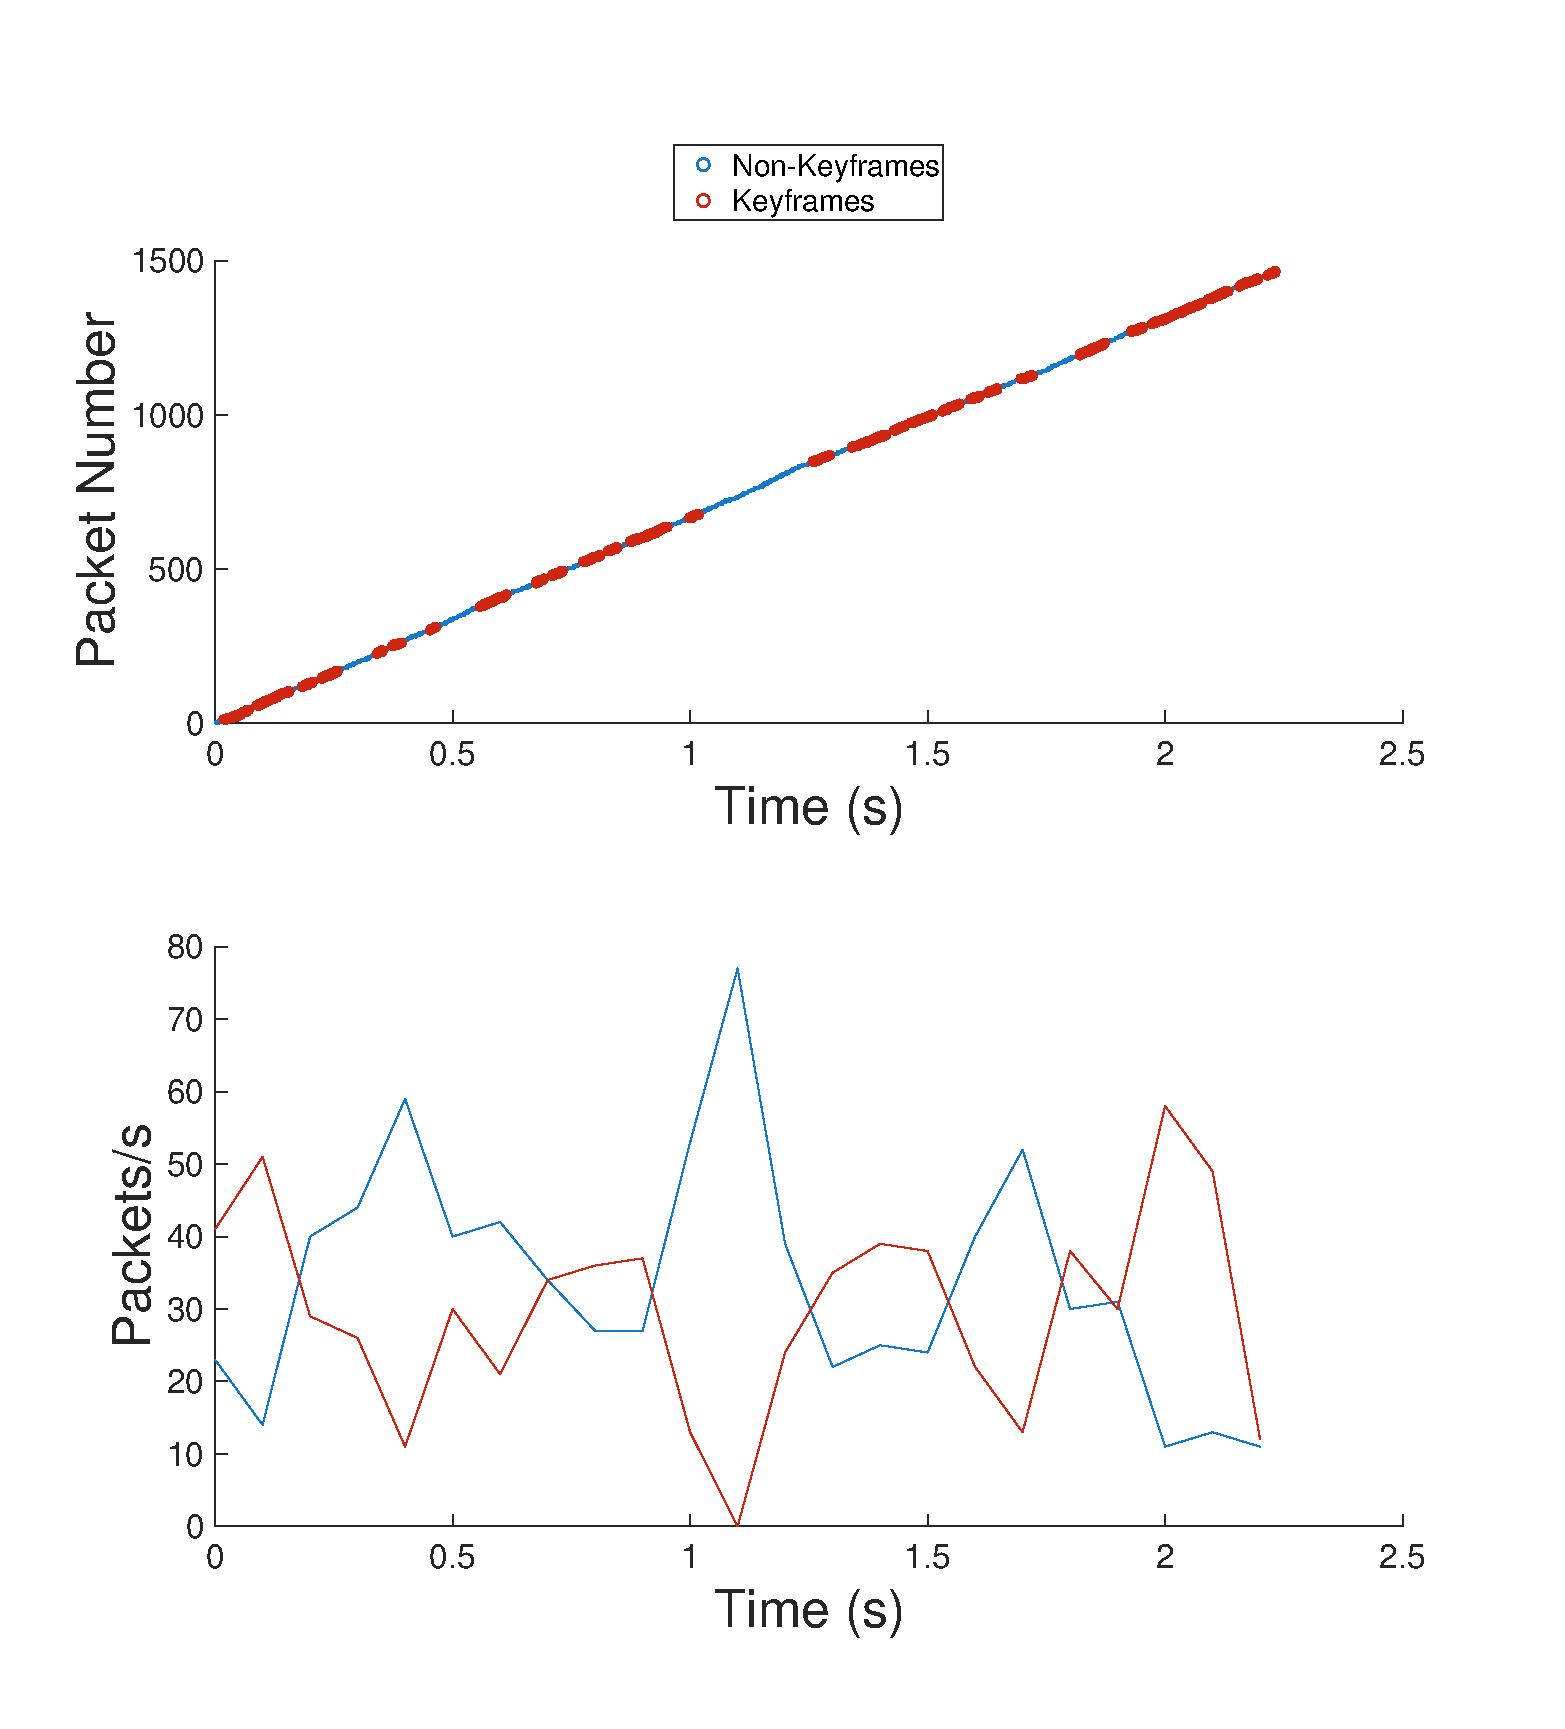
\includegraphics[scale = 0.55]{rand_slow_16_16_50}
\caption{Random cross-traffic ; Slow Channel (Path A : 16 Mbps, Path B : 16 Mbps), 50\% channel occupation, measured at the end of Path B}
\end{figure}

\begin{figure}[!h]
\centering
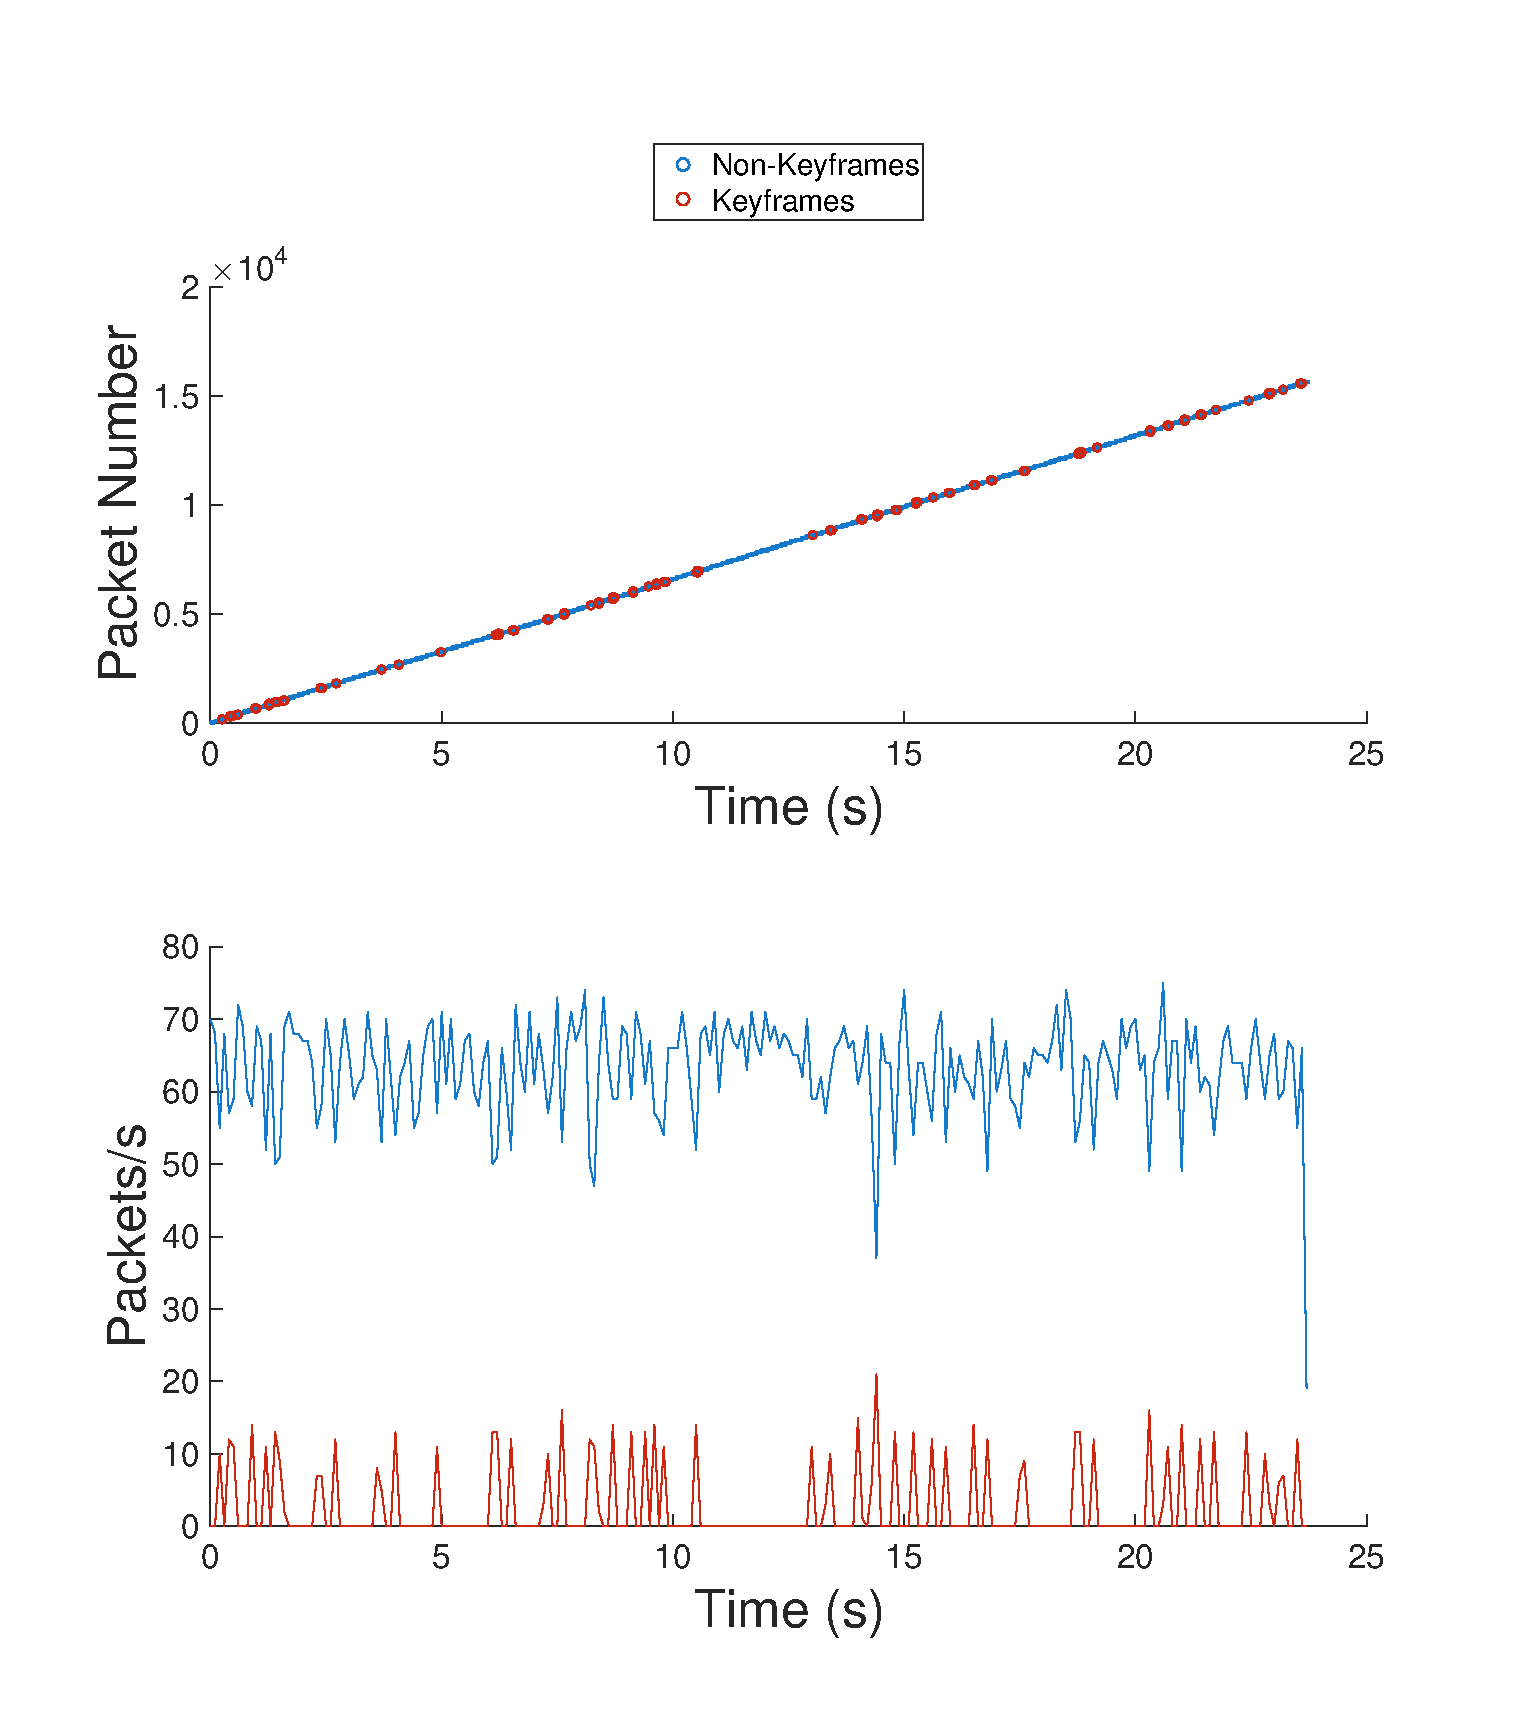
\includegraphics[scale = 0.55]{rand_med_16_16_50}
\caption{Random cross-traffic ; Medium Channel (Path A : 16 Mbps, Path B : 16 Mbps), 50\% channel occupation, measured at the end of Path B}
\end{figure}

\clearpage

\section{Sample Crosstraffic}

\begin{figure}[!h]
\centering
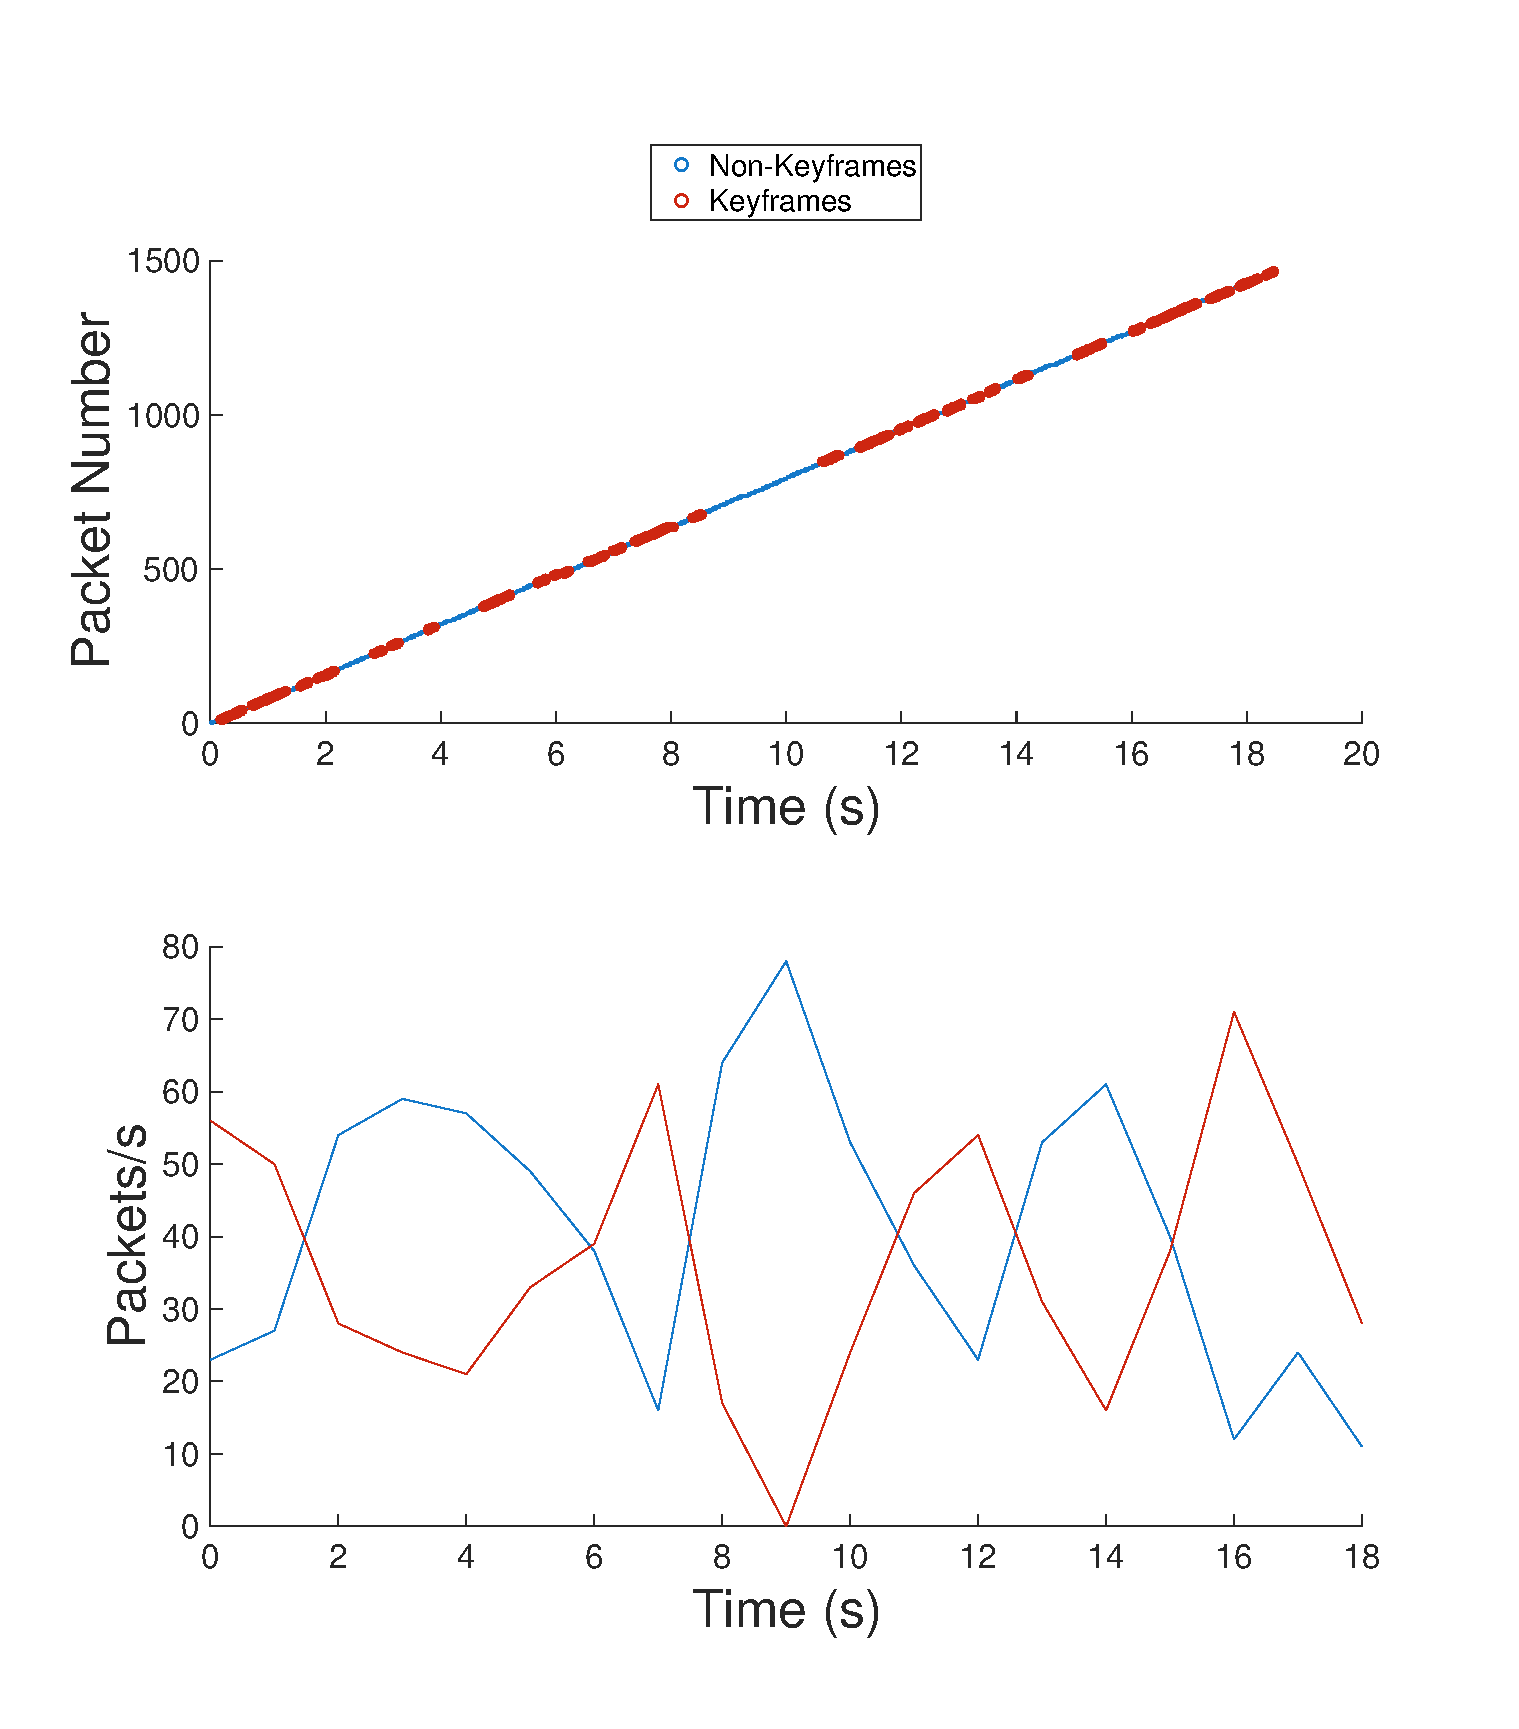
\includegraphics[scale = 0.55]{sample_slow_1_4}
\caption{Sample cross-traffic ; Slow Channel (Path A : 4 Mbps, Path B : 1 Mbps), measured at the end of Path B}
\end{figure}

\clearpage

\begin{figure}[!h]
\centering
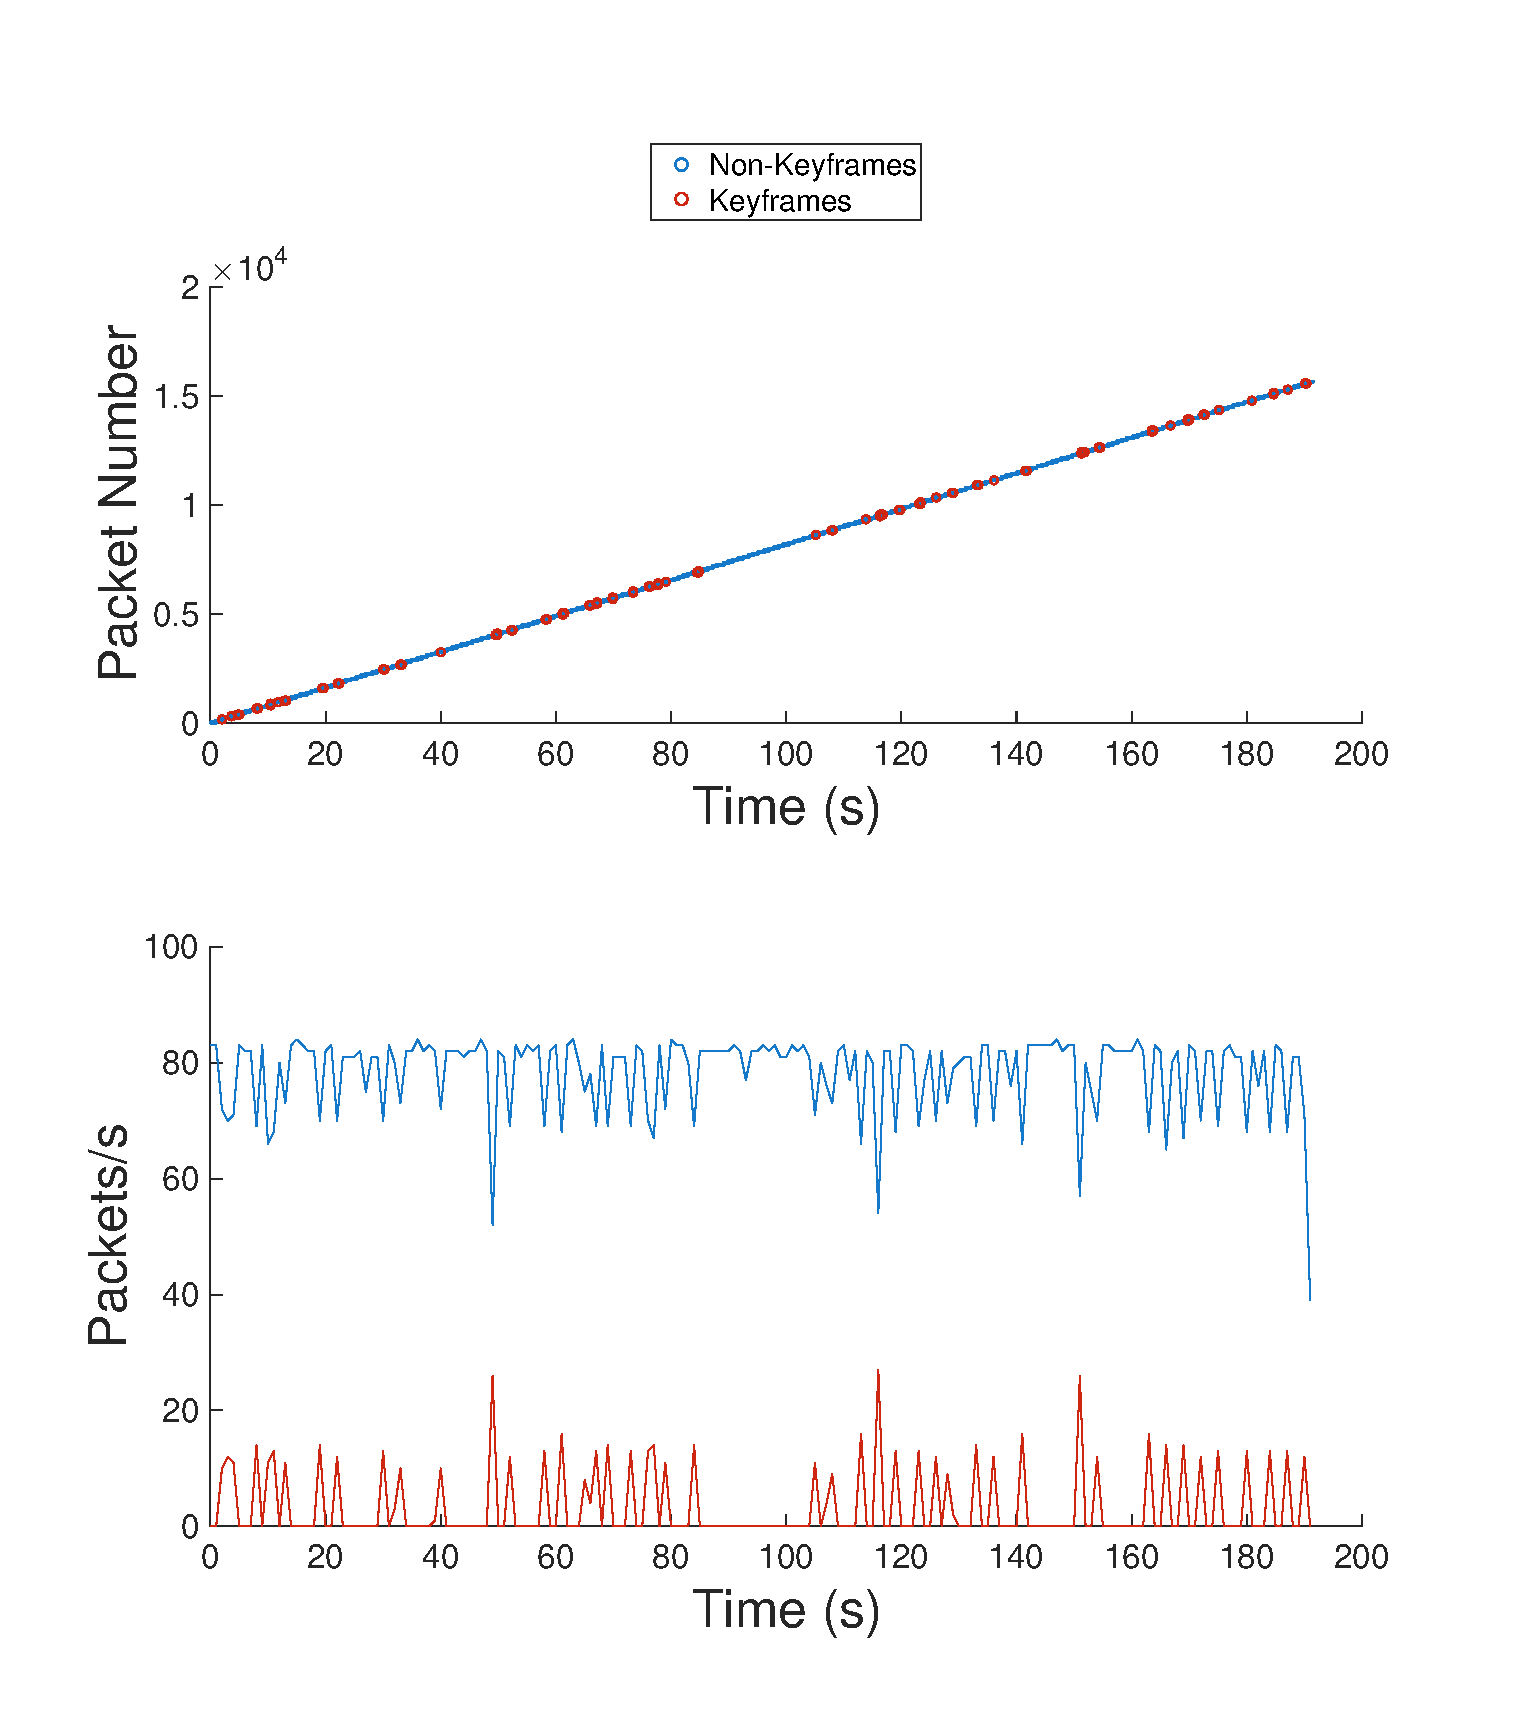
\includegraphics[scale = 0.55]{sample_med_1_4}
\caption{Sample cross-traffic ; Medium Channel (Path A : 4 Mbps, Path B : 1 Mbps), measured at the end of Path B}
\end{figure}

\begin{figure}[!h]
\centering
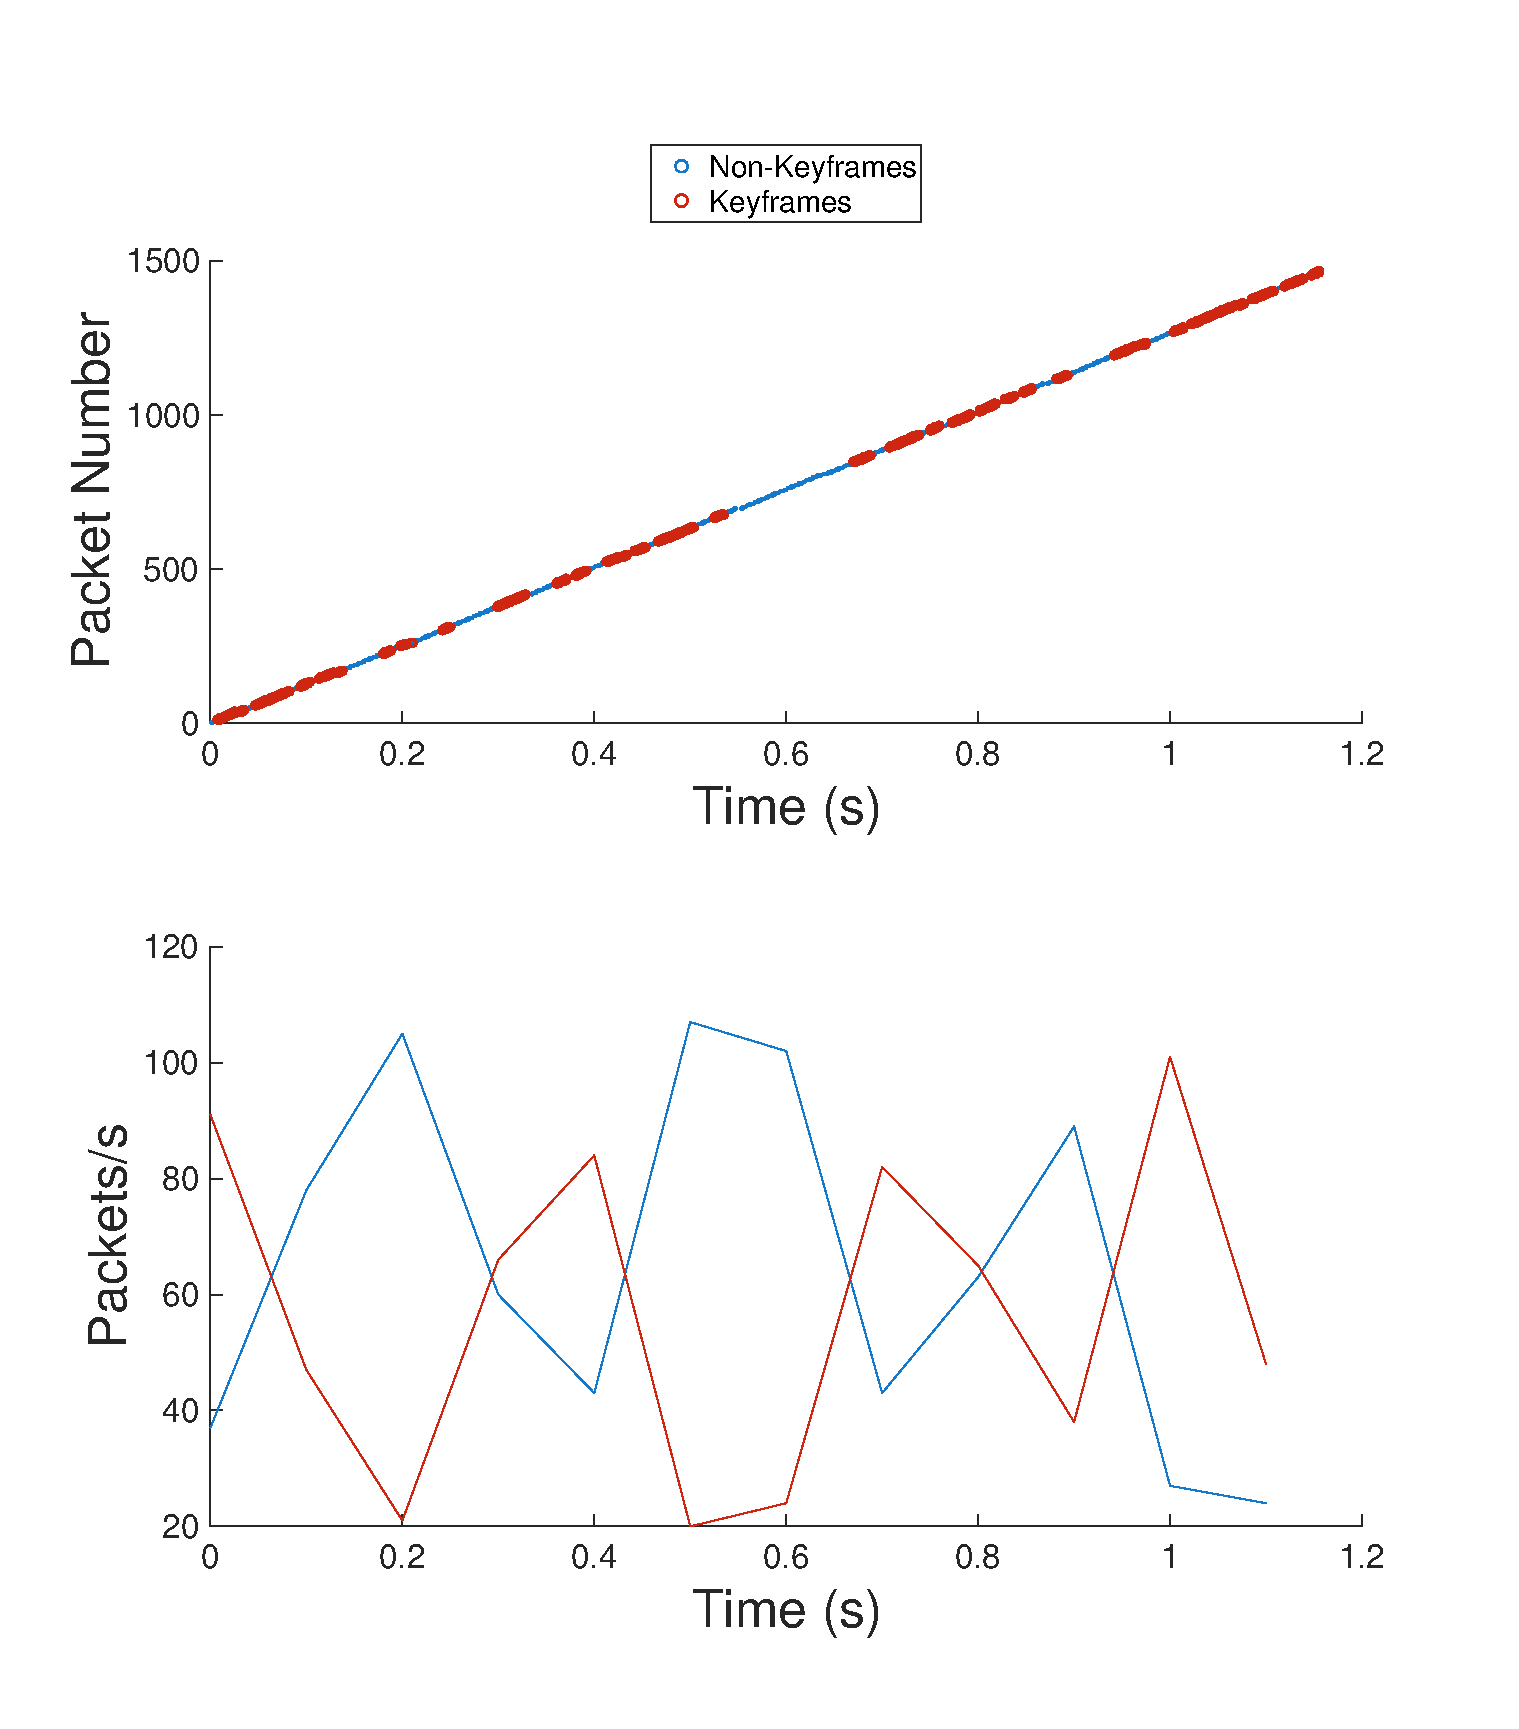
\includegraphics[scale = 0.55]{sample_slow_16_16}
\caption{Sample cross-traffic ; Slow Channel (Path A : 16 Mbps, Path B : 16 Mbps), measured at the end of Path B}
\end{figure}

\begin{figure}[!h]
\centering
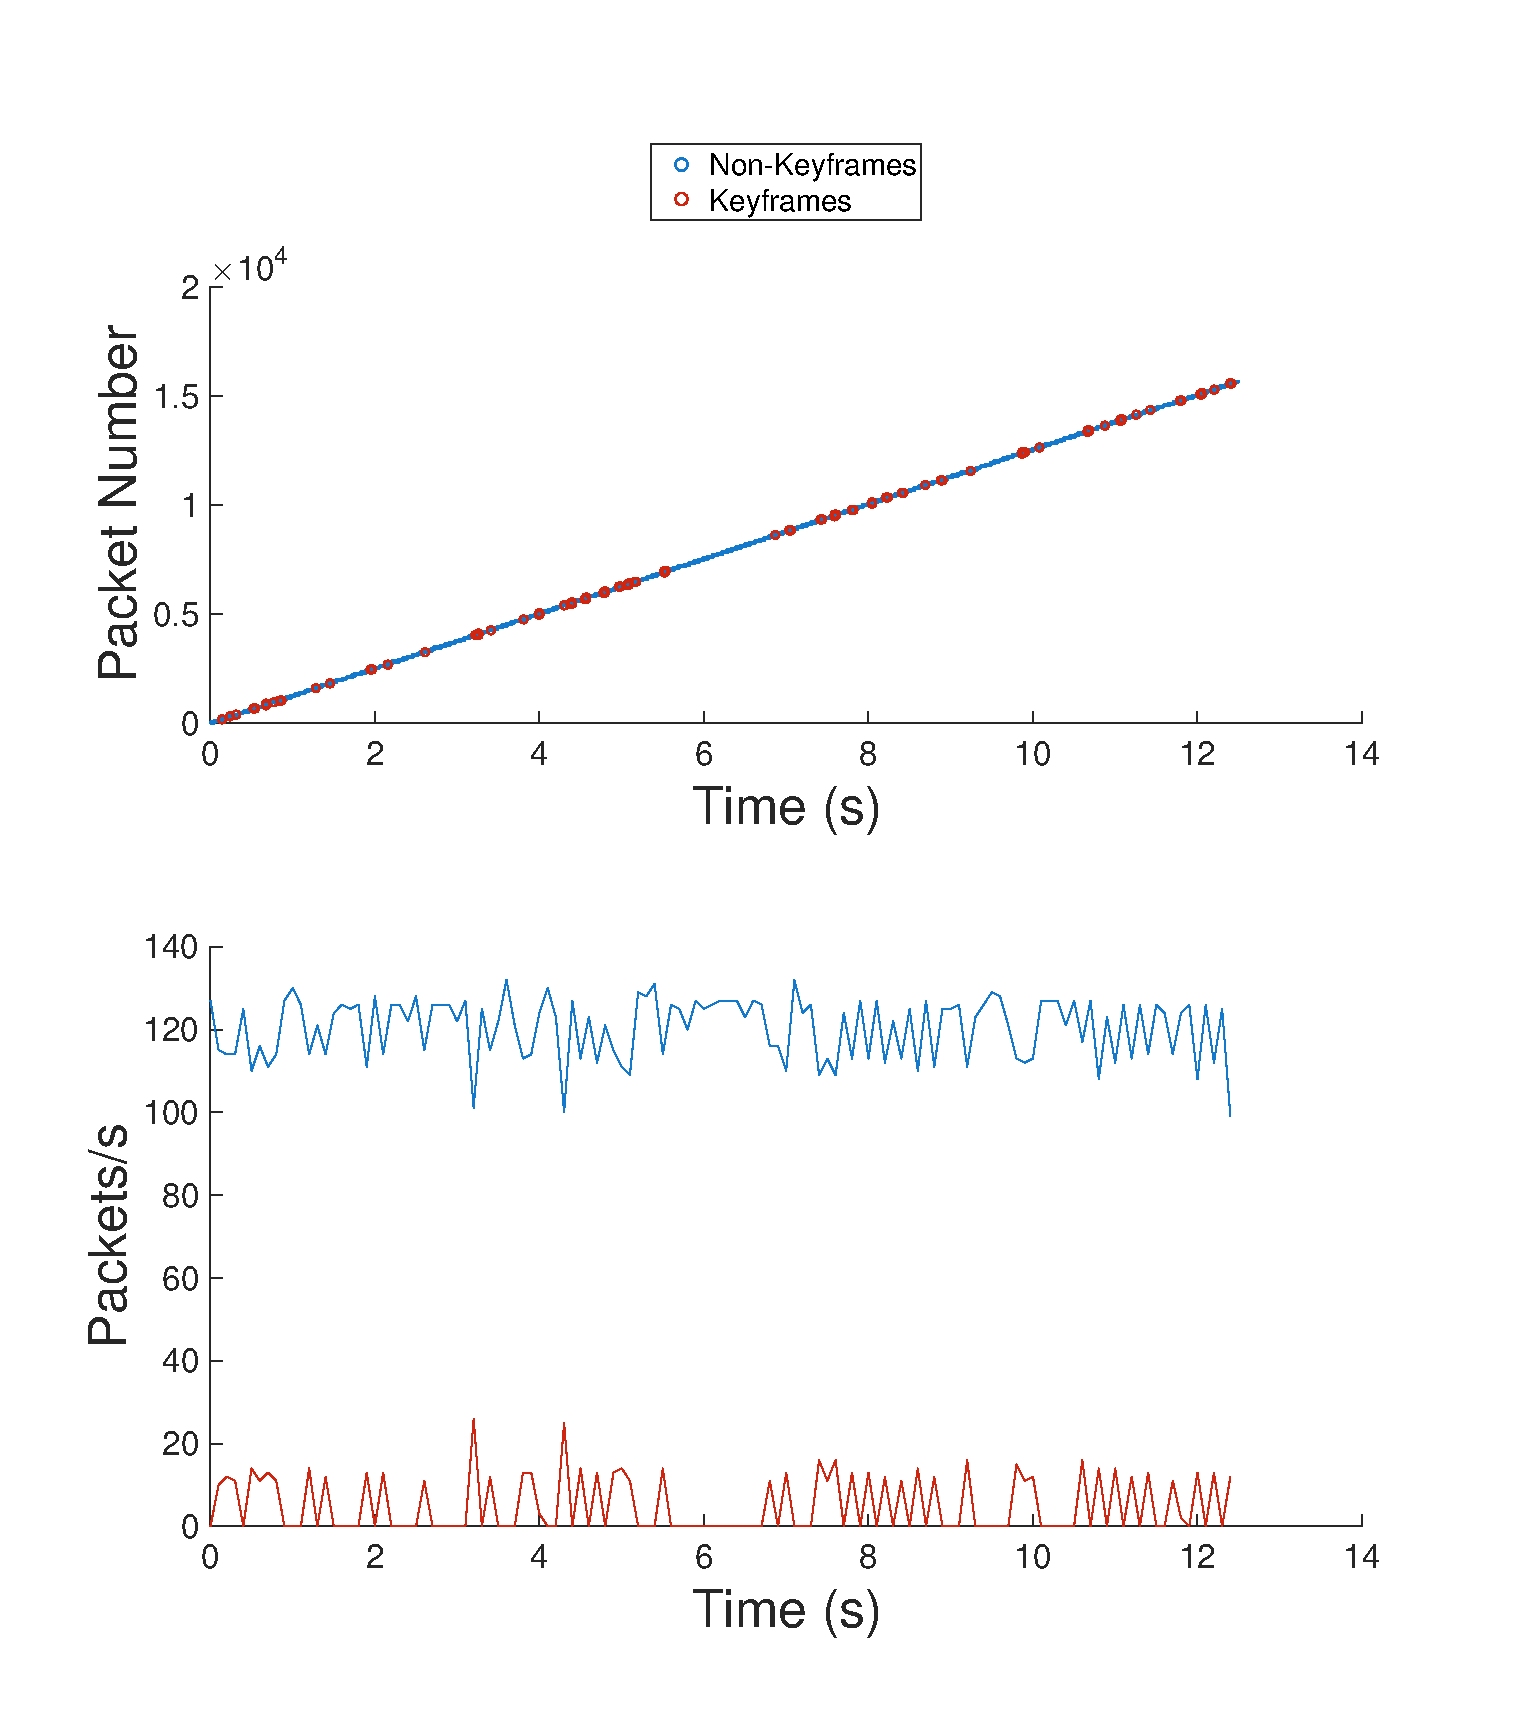
\includegraphics[scale = 0.55]{sample_med_16_16}
\caption{Sample cross-traffic ; Medium Channel (Path A : 16 Mbps, Path B : 16 Mbps), measured at the end of Path B}
\end{figure}